\begin{figure}[t]\centering
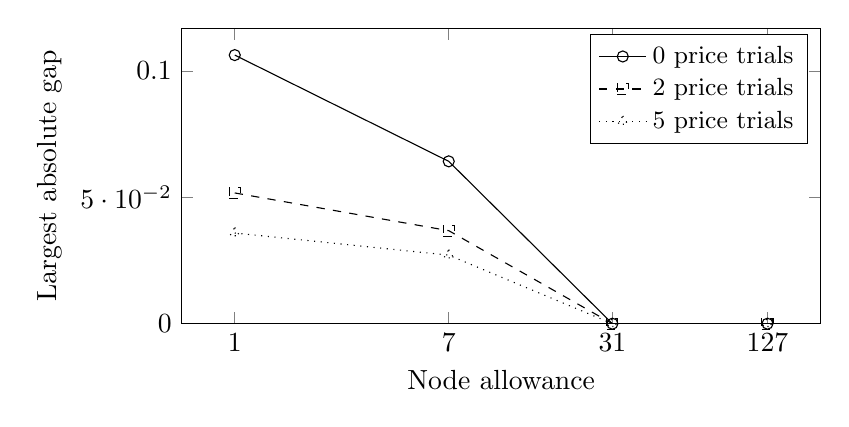
\begin{tikzpicture}\begin{axis}[width=.8\textwidth,height=2.1in,xmode=log,log basis x=2,xlabel={Node allowance},ylabel={Largest absolute gap},legend style={at={(.98,.98)},anchor=north east,font=\small},ymin=0,xtick={1,7,31,127},xticklabels={1,7,31,127}]
\addplot[solid,mark=o] coordinates {(1,0.10625) (7,0.0642181705229) (31,0) (127,0)};\addlegendentry{0 price trials}
\addplot[dashed,mark=square] coordinates {(1,0.0517181705229) (7,0.036796875) (31,0) (127,0)};\addlegendentry{2 price trials}
\addplot[dotted,mark=triangle] coordinates {(1,0.0358746189024) (7,0.0271215820313) (31,0) (127,0)};\addlegendentry{5 price trials}
\end{axis}\end{tikzpicture}
\caption{Node-budget and price sensitivity on the six fixed historical stress inputs. The vertical axis is the maximum rational interval width, converted to a display decimal only after verification. All requested budgets, including positive-width interruptions, contribute to the plot.}\label{fig:r51-nodes}
\end{figure}
